\clearpage

\section{MLP-Mixer}\label{sec:mlpmixer}\index{MLP-Mixer}

\begin{notebox}
\textbf{Paper: } \fullcite{phoo_self-training_2021}
\vspace{5pt}

\href{https://openreview.net/forum?id=EI2KOXKdnP}{reviews}
\hspace{1cm}
\href{https://github.com/lucidrains/mlp-mixer-pytorch}{code}
\hspace{1cm}
\href{run:/home/magda/Dropbox/Zot/Tolstikhin et al_2021_MLP-Mixer.pdf}{Local pdf}
\vspace{3pt}

Read with Simon\index{Simon} 24/2/2022
\hfill Notes taken: 1/3/2022 \index{March 2022}
\end{notebox}

\begin{notebox}[colback=red!5]
\tldr CNNs and attention-based models (vision transformers) are state of the art in high-dimensional computer vision problems but they are not necessary. MLP architecture with spatial and channel mixing uses standard MLP operations over data with transposed layout and can achieve similar results with at competitive training times and inference throughput capacity. So not beating anybody but showing that complex architectures are not necessary.
\end{notebox}

\begin{notebox}[colback=yellow!5]
\textbf{Notes:} 
\begin{itemize}[nosep]
\item Why exploring accuracy on downstream task with pre-training on ImageNet and ImageNet21-K and not directly on the ImageNet data? Would it not show so good results?
\item They claim CNN bring into the modeling inductive biases which they do not need. But their patch and channel based architecture and operations are also inductive biases. For normal tabular data or for sequences, these would have to be different.
\end{itemize}
\end{notebox}

CNNs and attention-based models (vision transformers) are state of the art in high-dimensional computer vision problems. Here they propose \iterm{MLP-mixer} which relies on standard MLP architecture with changes to data layout (reshapes and transpose).
It separates the per-location \iterm{channel mixing} and cross-location \iterm{token-mixing} operations (both simple MLPs with parameter sharing) and applies one after the other to each patch representation across the channels and then to each channel across the patch representations (the latter is simply applied to transposed data). The representation dimensions are preserved through these operations (though the inner MLP dimension can be different) so that there can be skip connections.

Most of the paper is about experiments - accuracy on downstream tasks with pre-training on ImageNet and ImageNet21-K.
MLP-Mixer has comparable accuracy to sota CNN and transformer models and at the same time high throughput at inference time and competitive training time.
Unlike CNN-based methods it is also resistant to within-patch pixel permutations and somewhat better adapted to full image permutations.
The extracted features at higher layers are simpler shapes with opposite phases, at deeper layers they have not apparent structure.

\begin{figure}[ht]
\centering
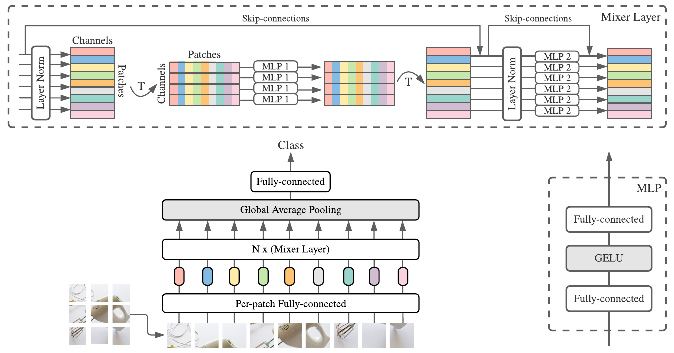
\includegraphics[width=0.9\textwidth]{mlpmixer_Figure1.png}
\caption{MLP-mixer: First all patches are linearly projected with the same projection matrix. Then multiple Mixer Layers are applied and with final global average pooling and fully connected layer for the classification.}
\end{figure}

